\documentclass{article}
\usepackage[a4paper,top=0.75in, bottom=0.75in, left=1in, right=1in,footskip=0.2in]{geometry}
%\usepackage{fullpage}
%-----------------Hyperlink Packages--------------------
\usepackage{hyperref}
\hypersetup{
	 colorlinks   = true,
     citecolor    = black,
     linkcolor    = black,
     urlcolor     = black
}
%-----------------Figure Packages--------------------
\usepackage{graphicx}                       % For figures
%\usepackage{epsfig} % for postscript graphics files
%------------------Math Packages------------------------
\usepackage{amssymb,amsmath}
\usepackage{textcomp}
\usepackage{mdwmath}
\usepackage{mdwtab}
\usepackage{eqparbox}
%------------------Table Packages-----------------------
\usepackage{rotating}                     % Used to rotate tables
\usepackage{array}                        % Fixed column widths for tables
%-----------------Algorithm Packages--------------------
\usepackage{listings}                     % Source code
\usepackage{algorithm}                    % Pseudo Code
\usepackage{algpseudocode}
%---------------------------------------------------------
\usepackage{pgf}
\usepackage{tikz}
\usepackage[utf8]{inputenc}
\usetikzlibrary{arrows,automata}
\usetikzlibrary{positioning}


\tikzset{
    state/.style={
           rectangle,
           draw=black,
           minimum height=2em,
           inner sep=2pt,
           text centered,
           },
}

\setcounter{tocdepth}{3}
%opening

\begin{document}

\title{
Course Project for Compilers \\
System Design
}
\author{Class 1, Team 10}
\date{\today}
\maketitle
\tableofcontents
\section{Team Members}

\begin{table}[H]
\centering
\begin{tabular}{l l l}
Name & Student ID  & Job\\
\hline
Fan Ziyao & 12330081 & Team leader, database implementation\\
Chen Zeyu & 12330056 & System implementation \\
Huang Long & 12330132 & Database implementation \\
Zhang Qiuyi (Class 2) & 12330402 & Frontend, documentation \\
Zhu Lichen (Class 2) & 12330439 & Testing
\end{tabular}
\end{table}

\section{System Design}

The system is divided into four parts, with functionalities shown in Figure~\ref{fig:sys}.

\begin{figure}[H]
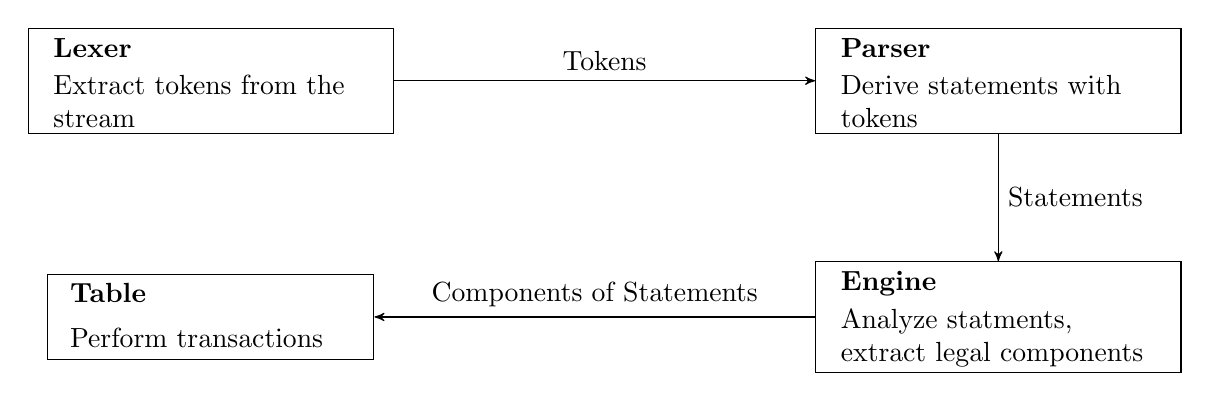
\begin{tikzpicture}[->,>=stealth']

 \node[state, text width=4.5cm] (LEXER) 
 {\begin{tabular}{l}
   \textbf{Lexer}\\[0.3em]
   \parbox{4cm}{Extract tokens from the stream
   }
  \end{tabular}};

 \node[state,
 node distance=10cm,
 text width=4.5cm,
 right of=LEXER,
 ] (PARSER)
 {\begin{tabular}{l}
    \textbf{Parser}\\[0.3em]
    \parbox{4cm}{Derive statements with tokens
    }
   \end{tabular}};
 
 \node[state,
 node distance=3cm,
 text width=4.5cm,
 below of=PARSER,
 ] (ENGINE)
 {\begin{tabular}{l}
     \textbf{Engine}\\[0.3em]
     \parbox{4cm}{Analyze statments, \\
     extract legal components
     }
    \end{tabular}};

 \node[state,
 left of=ENGINE,
 node distance=10cm,
 text width=4cm] (TABLE) 
 {\begin{tabular}{l}
      \textbf{Table}\\[0.3em]
      \parbox{4cm}{Perform transactions
      }
     \end{tabular}};


 \path (LEXER) edge node[anchor=east, above]
   {
   	Tokens
   } (PARSER)
   (PARSER) edge node[anchor=east,right]
   {
  	 Statements
   }(ENGINE)
   (ENGINE) edge node[anchor=east,above]
   {
     Components of Statements
   }(TABLE)
 ;
\end{tikzpicture}
\caption{System design}
\label{fig:sys}
\end{figure}

\section{Lexer Design}

\subsection {Token Specification}
\begin{align*}
num \quad\to\quad & \texttt{[0-9]+} \\
id \quad\to\quad & \texttt{[\_A-Za-z][\_A-Za-z0-9]*} \\
CREATE \quad\to\quad & \texttt{CREATE} \\
TABLE \quad\to\quad & \texttt{TABLE} \\
INT \quad\to\quad & \texttt{INT} \\
DEFAULT \quad\to\quad & \texttt{DEFAULT} \\
PRIMARY \quad\to\quad & \texttt{PRIMARY} \\
KEY \quad\to\quad & \texttt{KEY} \\
INSERT \quad\to\quad & \texttt{INSERT} \\
INTO \quad\to\quad & \texttt{INTO} \\
VALUES \quad\to\quad & \texttt{VALUES} \\
DELETE \quad\to\quad & \texttt{DELETE} \\
FROM \quad\to\quad & \texttt{FROM} \\
WHERE \quad\to\quad & \texttt{WHERE} \\
SELECT \quad\to\quad & \texttt{SELECT} \\
LT \quad\to\quad & \texttt{<} \\
GT \quad\to\quad & \texttt{>} \\
NEQ \quad\to\quad & \texttt{<>} \\
EQ \quad\to\quad & \texttt{==} \\
GEQ \quad\to\quad & \texttt{>=} \\
LEQ \quad\to\quad & \texttt{<=} \\
PLUS \quad\to\quad & \texttt{+} \\
MINUS \quad\to\quad & \texttt{-} \\
MUL \quad\to\quad & \texttt{*} \\
DIV \quad\to\quad & \texttt{/} \\
AND \quad\to\quad & \texttt{\&\&} \\
OR \quad\to\quad & \texttt{||} \\
NOT \quad\to\quad & \texttt{!} \\
COMMA \quad\to\quad & \texttt{,} \\
SEMICOLON \quad\to\quad & \texttt{;} \\
L\_PAREN \quad\to\quad & \texttt{(} \\
R\_PAREN \quad\to\quad & \texttt{)} \\
words \quad\to\quad & CREATE \quad | \quad TABLE  \quad | \quad INT \\
&| \quad DEFAULT \quad | \quad PRIMARY \quad | \quad KEY \quad \\
&| \quad INSERT \quad | \quad INTO \quad | \quad VALUES \quad \\
&| \quad DELETE \quad | \quad FROM \quad \\
&| \quad WHERE \quad | \quad SELECT \\
singleOp \quad\to\quad &
PLUS \quad | \quad MINUS \quad | \quad MUL \\
&| \quad DIV \quad | \quad L\_PAREN \quad | \quad R\_PAREN \\
&| \quad COMMA \quad | \quad SEMICOLON \\
ops \quad\to\quad &
AND \quad | \quad OR \quad | \quad NOT \quad | \quad LT \\
&| \quad GT \quad | \quad NEQ \quad | \quad EQ \quad | \quad GEQ \\
&| \quad LEQ \quad | \quad PLUS \quad | \quad MINUS \quad | \quad MUL \\
&| \quad DIV \quad | \quad L\_PAREN \quad | \quad R\_PAREN \\
&| \quad COMMA \quad | \quad SEMICOLON
\end{align*}
\subsection{DFA}

\section{Parser Design}

\subsection{Grammar}

\subsection{\texttt{First} Sets}
\begin{align*}
\textsc{first}(ssql\_stmt) & = \{CREATE, INSERT, DELETE, SELECT\} \\
\textsc{first}(create\_stmt) & = \{CREATE\} \\
\textsc{first}(decl\_list) & = \{id, PRIMARY\} \\
\textsc{first}(\_decl\_list) & = \{COMMA, \epsilon\} \\
\textsc{first}(decl) & = \{id, PRIMARY\} \\
\textsc{first}(default\_spec) & = \{DEFAULT, \epsilon\} \\
\textsc{first}(expr[simple=true]) & = \{PLUS, MINUS, num, L\_PAREN\} \\
\textsc{first}(expr[simple=false]) & = \{PLUS, MINUS, num, id\} \\
\textsc{first}(\_expr) & = \{PLUS, MINUS, \epsilon\} \\
\textsc{first}(term[simple=true]) & = \{PLUS, MINUS, num, L\_PAREN\} \\
\textsc{first}(term[simple=false]) & = \{PLUS, MINUS, num, id\} \\
\textsc{first}(\_term) & = \{MUL, DIV, \epsilon\} \\
\textsc{first}(unary[simple=true]) & = \{PLUS, MINUS, num, L\_PAREN\} \\
\textsc{first}(unary[simple=false]) & = \{PLUS, MINUS, num, id\} \\
\textsc{first}(column\_list) & = \{id\} \\
\textsc{first}(\_column\_list) & = \{COMMA, \epsilon\} \\
\textsc{first}(insert\_stmt) & = \{INSERT\} \\
\textsc{first}(value\_list) & = \{PLUS, MINUS, num, L\_PAREN\} \\
\textsc{first}(\_value\_list) & = \{COMMA, \epsilon\} \\
\textsc{first}(delete\_stmt) & = \{DELETE\} \\
\textsc{first}(where\_clause) & = \{WHERE, \epsilon\} \\
\textsc{first}(disjunct) & = \{L\_PAREN, NOT, PLUS, MINUS, num, id\} \\
\textsc{first}(\_disjunct) & = \{OR, \epsilon\} \\
\textsc{first}(conjunct) & = \{L\_PAREN, NOT, PLUS, MINUS, num, id\} \\
\textsc{first}(\_conjunct) & = \{AND, \epsilon\} \\
\textsc{first}(bool) & = \{L\_PAREN, NOT, PLUS, MINUS, num, id\} \\
\textsc{first}(comp) & = \{PLUS, MINUS, num, id\} \\
\textsc{first}(rop) & = \{NEQ, EQ, LT, GT, LEQ, GEQ\} \\
\textsc{first}(query\_stmt) & = \{SELECT\} \\
\textsc{first}(select\_list) & = \{MUL, id\} \\
\end{align*}

\subsection{\texttt{Follow} Sets}
\begin{align*}
\textsc{follow}(ssql\_stmt) =& \{\$\} \\
\textsc{follow}(create\_stmt) =& \{\$\} \\
\textsc{follow}(decl\_list) =& \{R\_PAREN\} \\
\textsc{follow}(\_decl\_list) =& \{R\_PAREN\} \\
\textsc{follow}(decl) =& \{COMMA, R\_PAREN\} \\
\textsc{follow}(default\_spec) =& \{COMMA, R\_PAREN\} \\
\textsc{follow}(expr[true]) =& \{COMMA, R\_PAREN\} \\
\textsc{follow}(expr[false]) =& \{NEQ, EQ, LT, GT, LEQ,\\
 & GEQ, AND, OR, SEMICOLON, R\_PAREN\} \\
\textsc{follow}(\_expr[true]) =& \{COMMA, R\_PAREN\} \\
\textsc{follow}(\_expr[false]) =& \{NEQ, EQ, LT, GT, LEQ,\\
& GEQ, AND, OR, SEMICOLON, R\_PAREN\} \\
\textsc{follow}(term[true]) =& \{PLUS, MINUS, COMMA, R\_PAREN\} \\
\textsc{follow}(term[false]) =& \{PLUS, MINUS, NEQ, EQ, LT, GT,\\
& LEQ, GEQ, AND, OR, SEMICOLON, R\_PAREN\} \\
\textsc{follow}(\_term[true]) =& \{PLUS, MINUS, COMMA, R\_PAREN\} \\
\textsc{follow}(\_term[false]) =& \{PLUS, MINUS, NEQ, EQ, LT, GT,\\
& LEQ, GEQ, AND, OR, SEMICOLON, R\_PAREN\} \\
\textsc{follow}(unary[true]) =& \{MUL, DIV, PLUS, MINUS, COMMA, R\_PAREN\} \\
\textsc{follow}(unary[false]) =& \{MUL, DIV, PLUS, MINUS, NEQ, EQ, LT,\\
& GT, LEQ, GEQ, AND, OR, SEMICOLON, R\_PAREN\} \\
\textsc{follow}(column\_list) =& \{FROM, R\_PAREN\} \\
\textsc{follow}(\_column\_list) =& \{FROM, R\_PAREN\} \\
\textsc{follow}(insert\_stmt) =& \{\$\} \\
\textsc{follow}(value\_list) =& \{R\_PAREN\} \\
\textsc{follow}(\_value\_list) =& \{R\_PAREN\} \\
\textsc{follow}(delete\_stmt) =& \{\$\} \\
\textsc{follow}(where\_clause) =& \{SEMICOLON\} \\
\textsc{follow}(disjunct) =& \{SEMICOLON, R\_PAREN\} \\
\textsc{follow}(\_disjunct) =& \{SEMICOLON, R\_PAREN\} \\
\textsc{follow}(conjunct) =& \{OR, SEMICOLON, R\_PAREN\} \\
\textsc{follow}(\_conjunct) =& \{OR, SEMICOLON, R\_PAREN\} \\
\textsc{follow}(bool) =& \{AND, OR, SEMICOLON, R\_PAREN\} \\
\textsc{follow}(comp) =& \{AND, OR, SEMICOLON, R\_PAREN\} \\
\textsc{follow}(rop) =& \{PLUS, MINUS, num, id\} \\
\textsc{follow}(query\_stmt) =& \{\$\} \\
\textsc{follow}(select\_list) =& \{FROM\} 
\end{align*}
\subsection{Parsing Table}

\section{Database Design}

\section{Complexity Analysis}

\end{document}
